% !TEX root = ../main.tex

%先介绍做课题的目的和背景,再引出需要用到COMSOL来进行仿真,再介绍COMSOL


\chapter{引言}

\section{分子通信概述}
\subsection{分子通信的基本原理}
分子通信(molecular communication)指的是以生物化学分子作为信息载体的通信技术\cite{Hiyama2010Molecular},是地球上最古老、
最普遍的通信机制之一。无论是对简单的单细胞生物,还是对复杂的多细胞动植物来说,分子通信都是维持它们生命必不可少的一环。
例如,许多细菌都会对它们邻居分泌的信号分子(information molecular)做出反应,以协调彼此的行为,并影响它们自身的运动、
产生抗生素、生成孢子等行为,这被成为群体感应。同样的,信号分子(例如信息素)
也广泛的存在于从低等的昆虫到高等的哺乳动物的日常交流中,并深深的影响了它们的行为。
信息素由个体释放,并指导群体里的其他个体前往觅食地,警告同伴有潜在的危险,
以及协调其他各种行为。此外,在多细胞动物体内,细胞与细胞之间也通过信号分子进行通信,
以完成相应的生理功能。例如,我们人体的神经系统中的电信号的传递,就是由神经递质(一种信号分子)
的释放与接收来完成的;在内分泌系统中,内分泌系统会向循环系统释放激素分子,
它作为一种信号分子被远端的目标细胞(靶细胞)所接收,从而完成细胞间的通信,调控靶细胞的行为\cite{Atakan2014Molecular}。

如图
~\ref{fig:molecular_communication_example}
所示,在分子通信中,我们将纳米级别的微小结构称为纳米机器(nano-machine)。
一个典型的分子通信的典型过程指的是由信息的发送方纳米机器(简称发送器,Transmitter)生成能被接收方纳米机器(简称接收器,Receiver)
识别并接收的信息分子(Information Molecule),并基于信息分子的物理或化学特性编码信息。
送器释放的信息分子通过流体(液体或气体)介质传送到接收器后,由接收器接收并以特定的方式解码信息这一过程\cite{基于扩散的分子通信与身体域纳米网络}
。
\begin{figure}[H]
    \centering
    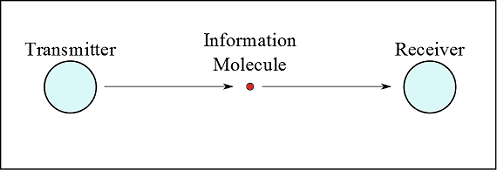
\includegraphics[scale=0.8]{simple model of molecular communication.png}
    \caption{分子通信示意图\cite{compic}}
    \label{fig:molecular_communication_example}
\end{figure}

\subsection{分子通信的发展现状}
分子通信这个概念在2005年被提出之后\cite{Suda05exploratoryresearch},经过十多年的发展,
已经在国际上成为了一个相当受关注的科研领域。

纳米技术与合成生物学的高速发展为纳米机器的设计与实现提供了新的思路。纳米技术能帮助研究者
在微小的尺度范围内制造能完成复杂功能的结构,如纳米碳管制造的能在细胞内进行药物输送
的精细结构\cite{drugDelivery}。合成生物学的目标是利用生物的基因表达功能,像计算机程序一样,
通过编程实现预定的功能。目前MIT的BioBrick项目已经建立了工程化的生物不见标准库\cite{Weiss_©2003}。

分子传输系统的设计与实现也是分子通信领域的研究重点。主要分为:1)基于自由扩散的传输系统。
这种方式主要利用溶液体系里的浓度梯度力来驱使信息分子自由扩散,不需要外加的能量源,系统简单,
适用于小尺度范围。2)基于分子马达的传输系统。这种方式使用了细胞内用于搬运特定物质的马达蛋白,
已实现物质的定向主动运输。类似的系统已经在人工环境下被广泛研究,如实现微管蛋白在预置的
显微光刻轨道网络上的可控运动\cite{HIRATSUKA20011555,QuickSystem}。3)长距离运输系统。高等动物体内的神经元细胞可以在
体内完成长距离的信号传递,如往返于膝盖与脊神经的膝跳反射信号。目前已经有研究设计了用于激活
跨膜离子信号传输的纳米机器以及用于连接不同神经元细胞的接口\cite{Balasubramaniam2011Development}。

目前分子通信的系统领域已经有多种概念模型和基本框架被建立,但还处于理论性研究阶段,技术水平较低\cite{achieveForMC},
还有很多的挑战等待研究人员,主要有:1)如何使纳米机器达到一个较高
的性能水平,使其能精确释放与接收信息分子。2)如何有效地传输信息分子,
如控制分子马达的运动等。3)如何扩大分子通信的通信距离与抗干扰能力\cite{zuo-peng2013review}。



\subsection{一种DNA分子受控释放的实现方法}
DNA分子中的磷酸基团会与$\ce{Zr^{4+}}$形成氢键,从而形成一种稳定的结构。通过逐层固定
DNA分子与$\ce{Zr^{4+}}$,我们可以得到两种物质逐层分部的结构。这被称为DNA/$\ce{Zr^{4+}}$
LbL(Layer-by-Layer,逐层)自组装结构\cite{Liu1999}。
文献\parencite{bm800766t,b812940a}中研究了电场控制下的
DNA/$\ce{Zr^{4+}}$LbL自组装结构分解,实现了DNA的可控释放。去除电势后电分解过程停止,
重新施加电势后电分解过程重新激活。组装的多层膜可以维持pDNA的连续释放,释放的DNA保留了其完整性和遗传活性。

\section{课题研究意义及内容}
\subsection{课题研究意义}
——引出本课题组的先前工作,指出为了更好地了解电压与DNA释放速度和释放浓度的关系,本课题开展对电压控DNA释放过程的建模。
\subsection{课题研究内容}
在课题组实验的基础上,探究DNA受控释放的原理。
综合电化学反应原理、化学动力学原理、扩散原理
等对DNA的受控释放过程进行建模与仿真。
根据仿真结果对影响该分子通信系统性能的参数进行
研究,并调整参数进行系统的优化。

\section{COMSOL Multiphysics多物理场仿真介绍}
\subsection{COMSOL Multiphysics的优势}
COMSOL Multiphysics是一个仿真平台,它最显著的特点和优势就是
多物理场问题的求解\cite{李淑君2014基于}。
可以实现从几何建模、定义材料属性、
设置物理场来描述物理现象,到求解模型的完整过程,
以及为提供准确可信的结果对模型的后处理。

多物理场是由大量偏微分方程(PDE)描述的,COMSOL Multiphysics
内置了这些约束方程,在
对多物理的建模与仿真时,只需要用户根据研究对象,选择合适的
偏微分方程或自定义方程,并进行组合,这样就可以实现多物理条件下的仿真\cite{王瑞2013基于}。

COMSOL Multiphysics的界面友好,操作灵活,仿真效果好,
而且在电气、化工、力学、流体等方面,有许多模板与案例,学习成本低。
还设置了与CAD、MATLAB这类软件联合编程的接口,这都使得COMSOL Multiphysics
成为一个应用广泛的有限元仿真软件。
\subsection{COMSOL Multiphysics的应用}
在分子通信的研究上,COMSOL Multiphysics也被大量运用。如\parencite{10.1007/978-3-319-67380-6_19}一文中
提到了在研究嵌入分子膜的纳米通信设备时,利用COMSOL Multiphysics对电场的分布进行
仿真。Sean McCutcheon与Robert Majeska等人在研究基于树突神经细胞的细胞间通讯装置时,
也用到了COMSOL Multiphysics对小分子扩散和流动状况进行仿真研究\cite{McCutcheon2017}。
在\parencite{10.1007/978-81-322-1007-8_56}一文中,研究者也使用了COMSOL Multiphysics
对纳米传感器的原理进行了建模仿真,并作为实验的对照,结果表明理论模型的结果与实际
实验结果最大误差为3\%。

